Secondary reactions integrate over a significant amount of information by their nature. In general, the primary product is born from a time-evolving spatially-varying plasma source. This alone creates complication, but it must further probe these varying plasma conditions as it streams through the plasma. The secondary particle ultimately depends on the state of the primary product at fusion which is influenced by all of these factors.

These complications motivate a model capable of creating and simulating the life of these primary products. Without simplification, the problem has $N=7$ dimensions; spatial position, velocity, and time. This motivates using a Monte Carlo approach to avoid the curse of dimensionality. 

\subsection{Monte Carlo Model for Tracing Particles Through a Plasma}

	A model has been created for creating and tracing arbitrary particles through arbitrary plasma conditions. This model is useful for many applications, but for our purposes can be used to generate secondary nuclear reactions by tracing primary nuclear products through a given plasma source. As of the writing of this thesis, the full code can by found at \url{https://github.com/bLahmann/MonteCarloParticleTracer}.
	
	In this model, a plasma is defined by several parameters. The first is the outer radius bound:
	%	
	\begin{equation}
		R_o(\theta, \varphi) = \sum_{\ell=0}^{\infty} \sum_{m=-\ell}^{\ell} \left(\Delta_{o}\right)_\ell^{m} \alpha_{\ell}^{m} \cos(m\varphi) P_{\ell}^{m}(\cos\theta)
		\label{eq:outerR}
	\end{equation}
	%
	where $\left(\Delta_{o}\right)_\ell^{m}$ are user-provided outer magnitudes (set equal to 0 if unspecified), $\alpha_{\ell}^{m}$ is a normalization factor given by:
	%
	\begin{equation}
		\alpha_{\ell}^{m} = \sqrt{\frac{2\ell+1}{4\pi}\frac{(\ell - m)!}{(\ell+m)!}}
	\end{equation}
	%
	and $P_{\ell}^{m}$ is an associated Legendre polynomials. Similarly, an inner radius bound is specified as:
	%	
	\begin{equation}
		R_i(\theta, \varphi) = \sum_{\ell=0}^{\infty} \sum_{m=-\ell}^{\ell} \left(\Delta_{i}\right)_\ell^{m} \alpha_{\ell}^{m} \cos(m\varphi) P_{\ell}^{m}(\cos\theta)
		\label{eq:innerR}
	\end{equation}
	%
	where $\left(\Delta_{i}\right)_\ell^{m}$ are user-provided inner magnitudes (set equal to 0 if unspecified). Plasma properties between the bounds are specified on a normalized radial grid $\hat{r}(r,\theta,\varphi)\in [0,1]$ defined by:
	\begin{equation}
		\hat{r}(r,\theta,\varphi) = \frac{r-R_{i}(\theta,\varphi)}{R_{o}(\theta,\varphi)-R_{i}(\theta,\varphi)}
	\end{equation}
	%
	The plasma properties are fully defined by a radial mass density $\rho(\hat{r})$, a radial ion temperature $T_{ion}(\hat{r})$, and a radial electron temperature $T_e(\hat{r})$. These are specified by the user as double arrays evaluated at user-specified points on the normalized radius grid. Finally, the plasma consists of an arbitrary number (>0) of plasma ion species. These are specified as a list of particle types (defined by their charges $\{Z_j\}$ and masses $\{M_j\}$) and a list of their corresponding number proportions \{$f_j$\} defined as:
	%
	\begin{equation}
		f_j = \frac{n_j(\hat{r})}{n(\hat{r})}
	\end{equation}
	%
	where $n_j$ is the number density of ion species $j$ and $n$ is the total number density.
	
	In this simplified specification model, a few key assumptions have been made. First is the separability of the plasma profiles. As specified, all profiles can only belong to a set of separable functions such that:
	%
	\begin{equation}
		\mathcal{F}(r, \theta, \varphi) = \mathcal{R}(r) \mathcal{G}(\theta, \varphi)
	\end{equation}
	%
	This assumption is made purely out of convenience as has no theoretical basis. The second assumption is that all plasma ion species have the same ion temperature profile $T_{ion}(\hat{r})$. That is, all ion species are always in thermal equilibrium. Finally we have assumed that number proportions $\{f_j\}$ are all constant throughout space. This disallows any ion-separation type modeling.
	
	The model requires that at least one plasma be fully specified. Additional plasmas can be added in \emph{layers} if desired. The model stacks these plasmas by forcing the inner boundary of every additional layer to be equal to the outer boundary of the layer before it. 
	
	Additionally the model requires that the user specify a particle source. The particle source is assumed to be born within the first specified plasma layer. The source is specified with a viable nuclear reaction (one that can occur between the plasma ion species in plasma layer) and a radial source distribution $N_{source}(\hat{r})$. Like plasma profiles this is defined with an array of doubles specifying the evaluated source density at specified values of $\hat{r}$. Alternatively, the user can provide a reactivity table $\left<\sigma v\right>_{source}(T_{ion})$ and the source profile will be automatically specified as:
	
	\begin{equation}
		N_{source}(\hat{r}) \propto \hat{r}^2 \rho(\hat{r})^2 \left<\sigma v\right>_{source}(T_{ion}(\hat{r}))
		\label{eq:burnDist}
	\end{equation}
	
	While this is information is sufficient for useful models to be run, additional information needs to be provided for secondary particle calculations. The model allows for an arbitrary number of nuclear reactions to be tracked in the simulation. To simulate secondary reactions, the appropriate secondary nuclear reaction (one that can occur between the source particle and ion species within specified plasma layers) needs to be specified. All nuclear reactions are specified by a list of reactant particle types, (specified by $Z$ and $M$), a list of product particle types, as well as a cross section table $\sigma(E_{COM})$, where $E_{COM}$ is the center of mass energy of the reaction. 
	
	The library comes with several pre-specified objects such as plasmas and nuclear reactions to aid in model specification. An example full specification routine using the Java API is shown in Figure \ref{MonteCarloCode}.
	
	\begin{figure}
	\begin{lstlisting}[language=java, basicstyle=\ttfamily\scriptsize]
import MonteCarloParticleTracer.*;

public class ExampleSetup {
	
  public static void main(String ... args) {
		
    // ******************** 
    // Plasma information *
    // ********************
	
    // Uniform profiles 
    double[] rhat = new double[]{0.0, 0.5, 1.0};        // Normalized units
    double[] rho = new double[]{1.0, 1.0, 1.0};         // Units g/cc
    double[] Tion = new double[]{4.0, 4.0, 4.0};        // Units keV
    double[] Te = new double[]{4.0, 4.0, 4.0};          // Units in keV
	
    // Outer radius information
    // Here we're setting an l=0 and l=2 mode
    int[] ells = new int[]{0, 2};
    int[] ms = new int[]{0, 0};
    double[] magnitudes = new double[]{50 * 1e-4, 0.1 * 50 * 1e-4};
	
	
    // ******************** 
    // Source information *
    // ********************

    // Prebuilt DDp reactivity table
    Reactivity sourceReactivity = Reactivity.DDp_Reactivity; 

    // Prebuilt D+D->T+p reaction 
    NuclearReaction sourceReaction = NuclearReaction.DD_t;               
	
    // Prebuilt D+T->n+a nuclear reaction
    NuclearReaction secondaryDTn = NuclearReaction.DT_n;            
	
	
    // ********************** 
    // Build the simulation *
    // **********************
	
    // Create the plasma object
    Plasma plasma = new Plasma(rhat, Tion, Te, rho);
    plasma.addSpecies(ParticleType.deuteron, 1.0);
    for (int i = 0; i < magnitudes.length; i++) {
      plasma.addOuterLegendreMode(ells[i], ms[i], magnitudes[i]);
    }
	
    // Create the model
    Model model = new Model("Example Model");
    model.addPlasmaLayer(plasma);
    model.setSourceInformation(sourceReaction, sourceReactivity);
    model.addNuclearReaction(secondaryDTn);
	
    // Run the model
    model.runSimulation((int) 1e6, 20);
	
  }
}
	\end{lstlisting}
	\caption{Example setup of the Monte Carlo Particle Tracer routine. In this simulation, the user has specified a deuterium plasma with uniform density and temperatures of 1.0 g/cc and 4.0 keV respectively. The plasma is a prolate spheroid and the source particles being traced are DD tritons. DT neutron reactions have been added to the model to simulate secondary DT neutrons resulting from the triton tracing.} 
	\label{MonteCarloCode}
	\end{figure}

	Each simulation consists of $N_p$ particles which can be distributed across $N_{CPU}$ number of processors specified by the user. Particles have their positions sampled from the specified radial source distribution and a polar distribution given by: 
	
	\begin{equation}
		f(\theta, \varphi) \propto \sin\theta \left(R_{o}(\theta, \varphi) - R_{i}(\theta, \varphi)\right)
	\end{equation}
	
	Their direction of travel are sampled randomly from a uniform spherical distribution and their energies are sampled from a normal distribution:
	%
	\begin{equation}
		f(E) = \mathcal{N}\left(\frac{m_D}{m_C+m_D}Q, \quad\frac{2m_Cm_D}{(m_A+m_B)(m_C+m_D)}QT_{ion}(\vec{r}_0)\right)
	\end{equation}
	%
	Where $m_A$, $m_B$, $m_C$ and $m_D$ are the masses specified in the source nuclear reaction, $Q$ is the energy gain of the specified source nuclear reaction, and $T_{ion}(\vec{r}_0)$ is the ion temperature evaluated at the birth position. Note that this formulation does not include up-shifts in the mean energy caused by the non-zero local temperature of the plasma. \cite{bibid} This approximation is thought to be more than sufficient for secondary particle applications although a more exact implementation would not require a great deal of work. All source particles are born with a weight:
	
	\begin{equation}
		w_{source}=\frac{1}{N_p}
	\end{equation}
	
	Particles then take steps through their current plasma layer until they reach a boundary or they lose all of their energy. The length of any given step is given by:
	%
	\begin{equation}
		\delta x_j = \frac{\min\left[L, \quad\frac{E_0}{(dE/dx)_j}\right]}{N_{STEPS}}
	\end{equation}
	%
	Where $L$ is the distance between the starting position and plasma layer boundary, $E_0$ is the birth energy of the particle being traced, $(dE/dx)_j$ is the local stopping power of the particle with the plasma layer evaluated at it's current position, and $N_{STEPS}$ is a hard coded integer set sufficiently large to resolve the plasma but sufficiently small so as to minimize computation time. Current implementations take $N_{STEPS}=50$. This flexible step length ensures smaller steps are taken to resolve details when $dE/dx$ is large. Future implementations may also want to have step sizes based on profile gradients as well to ensure profile information is resolved when gradients are sharp.
	
	It should be noted that calculating $L$ for any given position $\vec{r}$ and direction $\vec{\Omega}$ is itself a non-trivial calculation. Additionally, it must be computed several times ($\mathcal{O}(N_p\times N_{STEPS})$ for secondary calculations) so the calculation must be computationally efficient. Currently, the model uses a bisection method approach with the initial guess being:
	
	\begin{equation}
		L_0=\left(R_o(\vec{\Omega}) - R_i(\vec{\Omega})\right)
	\end{equation}
	
	One problem with this method, is it is not guaranteed to return the smallest solution if there are more than one. In other words, the method fails for concave boundaries. One way to fix this is to simply choose $L_0$ sufficiently small ($\sim \delta x$) to correctly resolve any concavities in the plasma. Unfortunately, this causes noticeably large increases in computation time due to the increased iteration requirement of the bisection method. Finding a more elegant solution to this problem would be of great benefit to the simulation algorithm. 
	
	With every step, a variety of routines are performed. The particles position is updated based on the step size, the particles energy is updated based on the local plasma stopping power, and a nuclear particle is born for every viable nuclear reaction added to the simulation. These product particles are born at the position of their parent with weight equal to:
	%
	\begin{equation}
		w_{product}=w_{parent} \mathbb{P}_{j}
	\end{equation}
	%
	where $w_{parent}$ is equal to the weight of the parent particle and $\mathbb{P}_{j}$ is the probability of the parent particle having a nuclear reaction during the current step given by:
	%
	\begin{equation}
		\mathbb{P}_{j} = n_{j} \sigma_{j} \delta x_j \left(1 - \mathbb{P}_{tot}\right)
	\end{equation}
	%
	where $n_j$ is the average number density of the reacting species evaluated over this step, $\sigma_{j}$ is the average cross section between the traced particle and the reacting plasma species evaluated over this step, and $\mathbb{P}_{tot}$ is the running total reaction probability for this particle given by:
	%
	\begin{equation}
		\mathbb{P}_{tot} = \sum_{k=0}^{j} \mathbb{P}_k
	\end{equation}

	To determine the value of $\sigma_j$, a background particle is sampled from the appropriate plasma species. It's direction is sampled from a random spherical distribution and it's energy is sampled from a Maxwell distribution:
	
	\begin{equation}
		f(E) \propto \sqrt{E} \exp \left[ - \frac{E}{T_{ion}(\hat{r})}\right]
	\end{equation}
	
	The energy of the product particle is given by:
	
	\begin{equation}
		E_C = \frac{1}{2} m_C |\vec{v}_C|^2
	\end{equation}
	%
	where $\vec{v}_C$ is the lab frame velocity and this time $m_C$ is the mass of the product particle from the specified nuclear reaction. Note that the product nuclear reaction is not necessarily equivalent to the source nuclear reaction. The lab frame velocity is given by:
	%
	\begin{equation}
		\vec{v}_C = \vec{u}_C + \vec{v}_{CM}
	\end{equation}
	%
	where $\vec{u}_C$ is the center of mass velocity of the product particle and $v_{CM}$ is the system's center of mass velocity given by:
	%
	\begin{equation}
		\vec{v}_{CM} = \frac{m_A\vec{v}_A + m_B\vec{v}_B}{m_A + m_B}
	\end{equation}
	%
	Where $m_A$ and $\vec{v}_A$ are the mass and velocity of the background particle and $m_B$ and $\vec{v}_B$ are the mass and velocity of the traced particle. The magnitude of $\vec{u}_C$ is given by:
	%
	\begin{equation}
		|\vec{u}_C| = \sqrt{\frac{2\mathcal{E}_C}{m_C}}
	\end{equation}
	%
	where $\mathcal{E}_C$ is the center-of-mass energy of the product particle given by:
	\begin{equation}
		\mathcal{E}_C = \frac{m_D}{m_C+m_D} \left(Q + K\right)
	\end{equation}
	%
	where $Q$ is the energy gain of the product reaction given by:
	\begin{equation}
		Q = \left(m_A + m_B - m_C - m_D\right)c^2
	\end{equation}
	%
	where $c$ is the speed of light, and $K$ is the kinetic energy given by:
	%
	\begin{equation}
		K = \frac{1}{2}\mu \left(\vec{v}_A - \vec{v}_B\right)^2
	\end{equation}
	%
	and $\mu$ is the reduced mass given by:
	\begin{equation}
		\mu = \frac{m_A m_B}{m_A + m_B}
	\end{equation}

	In default operations, $\vec{u}_C$ is sampled randomly from a uniform spherical distribution. In reality, the direction should be sampled from the differential cross section $(\frac{d\sigma_{j}}{d\Omega})$ but this feature is not currently implemented. Such details are not important for the secondary reactions discussed in this work because the differential cross section is nearly uniform. However, such details are required for other applications such as \emph{knock-on deuterons} \cite{bibid} that make adding this feature in the future desirable.
	
	Alternatively, the user can specify the direction of $\vec{v}_C$ (such that products only go to a detector of interest) when setting up the model. In this case, it is possible to calculate the magnitude of $\vec{v}_C$ without knowing the direction of $\vec{u}_C$ by using the law of cosines:
	
	\begin{equation}
		|\vec{u}_C|^2 = |\vec{v}_C|^2 + |\vec{v}_{CM}|^2 - 2\left(\vec{v}_C\cdot\vec{v}_{CM}\right)
	\end{equation}

	It is important to note that forcing the direction like this, results in non-physical distributions of $\vec{u}_C$. To correct this bias, the weight of the product particle needs to be multiplied by a correction term: \cite{bibid}
	
	\begin{equation}
		w^*_{product} = w_{product} \left(\frac{E_C}{\mathcal{E}_C}\right)
	\end{equation}  

	This correction term is, in itself, an approximation to the real correction. While the approximation holds for $|\vec{v}_C|\gg|\vec{v}_B|$, implementing the correct term would not require a great deal of additional work.
	
	After having it's direction and energy set, the parent particle routine pauses and the product particle begins tracing through the plasma. This process continues recursively until all of the original $N_p$ particles are traced. 
	
	We take a moment to note that every single particle produces on the order of $N_{STEPS}$ secondary particles instead of the more physical case of $\sim n\sigma R$.  This is valid because we are weighting the products according to the probability that they could have existed. This approach is useful because $n\sigma R \ll 1$ meaning we would have to sample many source particles just to tally a single secondary reaction. With the current algorithm, meaningful spectra can be produced with $N_p$ as low as $10^4$. 


\subsection{Profile Effects}

	With the model, we can investigate the impact that temperature and density profiles have on the observables. There are a handful of common models we can use to do this. The first commonly used model is the \emph{Hot Spot Model}. In this model temperature and densities are taken to be uniform throughout the plasma. Instead of following the burn distribution, all particles are born at the center of the plasma. That is:
	%
	\begin{equation}
		N_{source}(\hat{r}) = \delta_r(0);
	\end{equation}
	%
	where $\delta_r$ is the Dirac delta function. Every other model discussed will use equation \ref{eq:burnDist} to describe the source birth profile. 
	
	All models we consider (including the Hot Spot Model) have a temperature profile such that:
	%
	\begin{equation}
		T_{ion}(\hat{r})=T_{e}(\hat{r}) \propto \left(1 - \hat{r}^2\right)^\gamma
		\label{eq:tempProfile}
	\end{equation}
	%
	where $\gamma$ is just some exponent describing the peakedness of the profile. When $\gamma=0$, the model is referred to as the \emph{Uniform Model} because the temperature profiles are uniform. 
	
	The magnitude of the temperature profiles is set by the burn averaged temperature given by:
	%
	\begin{equation}
		\left<T\right>_{burn} = \frac{\int_{V} dV \rho^2 \left<\sigma v\right>_{source} T_{ion}}{\int_{V} dV \rho^2 \left<\sigma v\right>_{source}}
	\end{equation}


	\subsubsection{Yield Ratios}
	
	    \begin{figure}[h!]
	        \centering
	        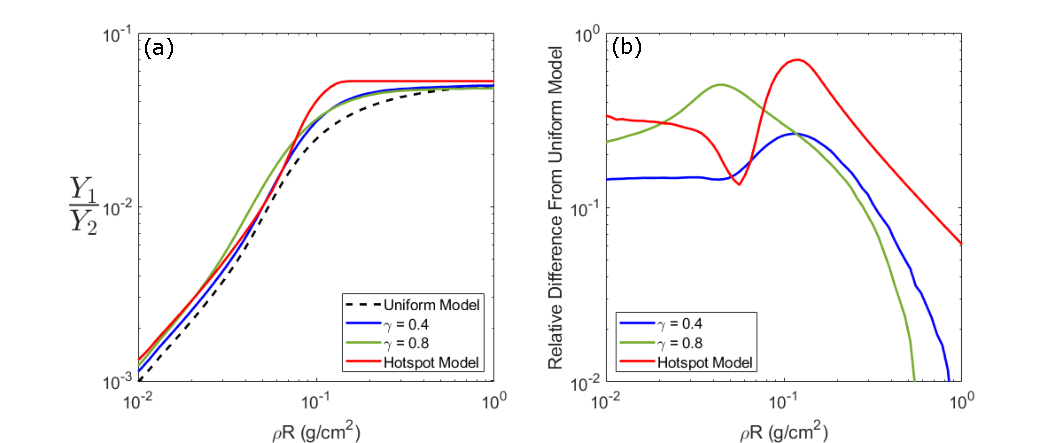
\includegraphics[scale=0.9]{Figures/yieldRatioProfiles.pdf}
	        \caption[Profile Effects on Yield Ratios]{Effects of temperature profiles on the observed yield ratio. All simulations had a burn averaged ion temperature of 4.0 keV and a uniform mass density of 1.0 g/cc. Figure \ref{fig:yieldRatioProfiles}(a) shows the actual yield ratios and Figure \ref{fig:yieldRatioProfiles}(b) shows the difference in the yield ratios compared to the uniform model. }
	        \label{fig:yieldRatioProfiles}
	    \end{figure}
	    
	    Figure \ref{fig:yieldRatioProfiles} shows the effects of these temperature profiles on the observed yield ratio. In general, adding a temperature profile increases the yield ratio. Alternatively, for a fixed yield ratio the inferred areal density is lower if one assumes a temperature profile. 
	    
	    This observation makes sense because temperature profiles force particles to be born more toward the center of the plasma. This means particles will see more areal density on average and thus increase the amount of secondary DT reactions. Notice that all models converge toward each other as the areal density is increased; this is because eventually there is enough areal density to stop any triton, regardless of where it is born. 
	    
	    The Hotspot Model can be thought of as an approximation of the most extreme case of this efect. All particles being born at the center is analogous to having $\gamma=\infty$. Note though, that the temperature profile cases actually have higher yield ratios than the Hotspot model in certain areal density regimes despite their finite peakedness. This is because the colder fuel is stopping the tritons more effectively, increasing the effective cross section as they slow down. This effect is not captured in the Hotspot approximation. 
	    
	    To comment briefly on how realistic these models are, we point to the Prav model \cite{bibid} and the Betti model \cite{bibid} which use $\gamma$ of 0.331 and 0.4 respectively. We note that the Betti model is slightly more complicated than equation \ref{eq:tempProfile}. The Uniform Model approximates $\gamma=0.4$ within 20\% accross the entire areal density regime. 
	
	\subsubsection{Spectra}
	
	    \begin{figure}[h!]
	        \centering
	        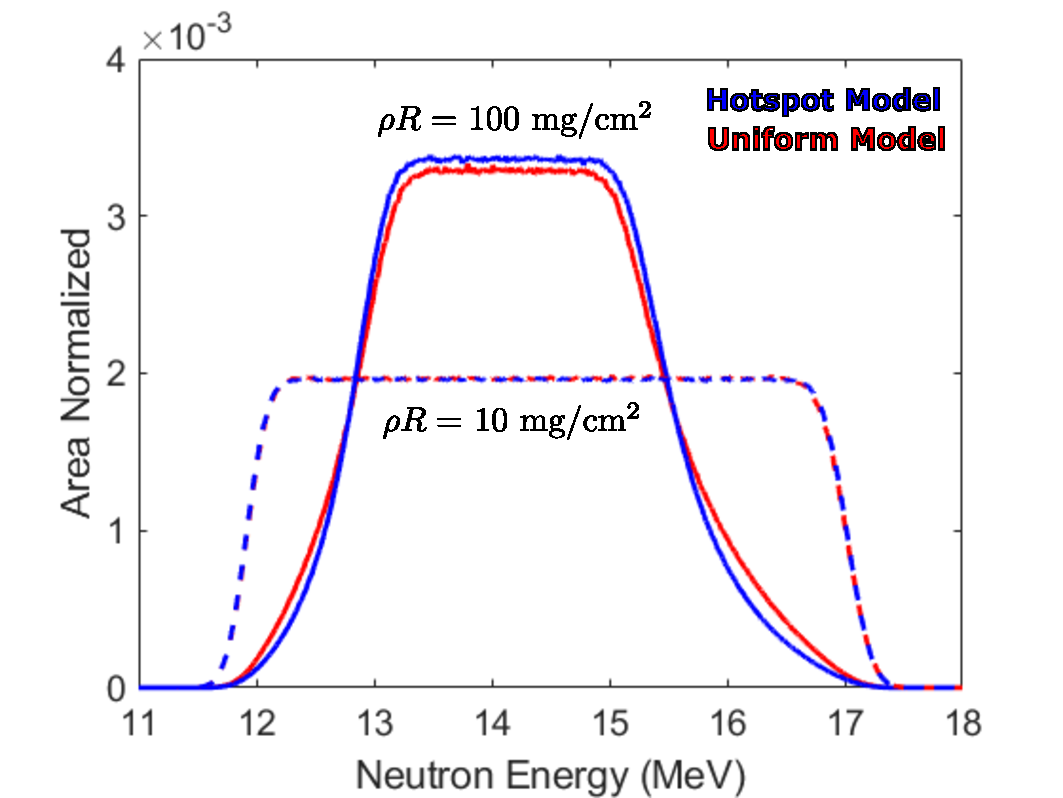
\includegraphics[scale=0.8]{Figures/spectraProfileEffects.pdf}
	        \caption[Profile Effects on Spectra]{Secondary DTn spectra simulated from a Hotspot Model (blue) and a Uniform Model (red). The dashed and solid curves correspond to areal densities of 10 and 100 mg/cm$^2$ respectively. All simulations were done with a uniform temperature and density of 4.0 keV and 1.0 g/cc respectively.}
	        \label{fig:spectraProfiles}
	    \end{figure}
	    
	    Figure \ref{fig:spectraProfiles} shows the effects of temperature profiles on the observed secondary spectra by highlighting the two most extreme cases. While both the Uniform Model and the Hotspot Model technically share the same profiles, the Hotspot Model is a proxy for a very peaked profile. One can show that the conclusions below do not change for finite valued $\gamma$.
	    
	    In general, very little change is seen in the spectra. It should be noted that the amplitudes change (as shown in Figure \ref{fig:yieldRatioProfiles}) with model. Additionally the exact transition behavior between the dashed and solid curve cases varies slightly. On either side of the areal density transition though, the spectra are nearly identical regardless of the temperature profiles. 
	    
	    This largely makes sense because the shape is much more sensitive to asymmetries and not global characteristics. So long as the tritons see the same plasma conditions in every direction, one can expect the secondary DT neutron spectra to be uniform in nature. 
	    

\subsection{Asymmetry Effects}

	\subsubsection{Yield Ratios}
	
	    For asymmetries, the areal density is a function of direction which makes comparisons slightly more tricky. In order to compare yield ratios, we will define a direction averaged areal density as:
	    
	    \begin{equation}
	        \left<\rho R\right> &= \frac{1}{4\pi}\int d\Omega \int dr \rho (r, \theta, \varphi)
	        \label{eq:dirAveragedRhoR}
	    \end{equation}
	    
	    We also define a convention for classifying asymmetry magnitudes widely used in the ICF community. In this convention we refer to $\ell$ mode asymmetries as $P\ell$ (not to be confused with the Legendre polynomials $P_\ell^m(\cos\theta)$) and they are defined as:
	    
	    \begin{equation}
	        P0 \equiv (\Delta_o)_0^0 \alpha_0^0
	        \label{eq:P0}
	    \end{equation}
	    
	    \begin{equation}
	        P\ell \equiv (\Delta_o)_\ell^0 \quad \ell \ne 0
	        \label{eq:Pl}
	    \end{equation}
	    
	    Note very importantly, that there is an inconsistency between P0 and all other P$\ell$. Often times we like to express P$\ell$ as a fraction of P0, so much so that several sources will omit P0. For example, P2 = 40\% would be equivalent to the more complete statement P2/P0 = 40\%. 
	    
	    \begin{figure}[h!]
	        \centering
	        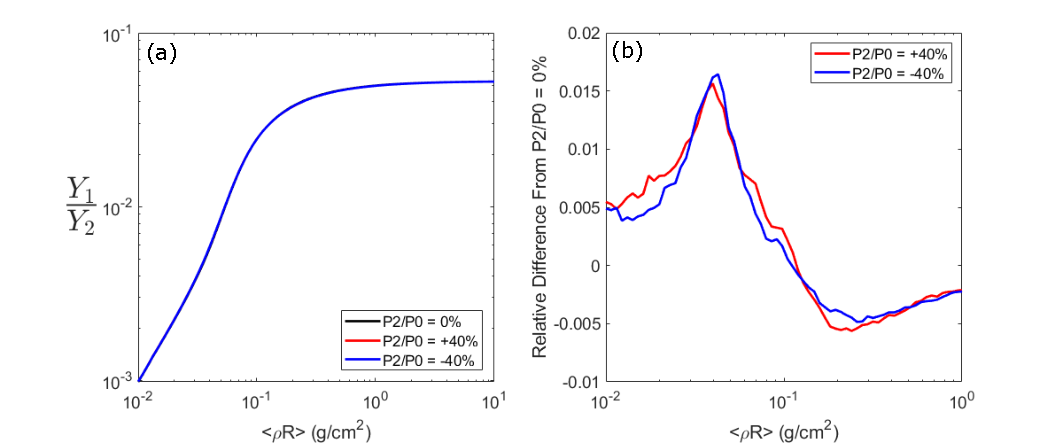
\includegraphics[scale=0.9]{Figures/yieldRatioAsym.pdf}
	        \caption[Asymmetry Effects on Yield Ratios]{Effects of asymmetries on the yield ratio. All simulations had a uniform temperature and density of 4.0 keV and 1.0 g/cc respectively. The black, red, and blue curves correspond to a P2/P0 of 0\%, 40\%, and -40\% respectively. Figure \ref{fig:yieldRatioAsym}(a) shows the actual yield ratios while Figure \ref{fig:yieldRatioAsym} shows relative differences in yield ratio compared to the P2/P0 = 0\% case.}
	        \label{fig:yieldRatioAsym}
	    \end{figure}
	    
	    Figure \ref{fig:yieldRatioAsym} shows that asymmetries have little to no effect on the inferred yield ratios when plotted against the direction averaged areal density. This is an extremely important result, as it means we can infer the average areal density without considering the many asymmetries that may be present in a real experiment.

	\subsubsection{Spectra}
	
	\begin{figure}[h!]
	    \centering
	    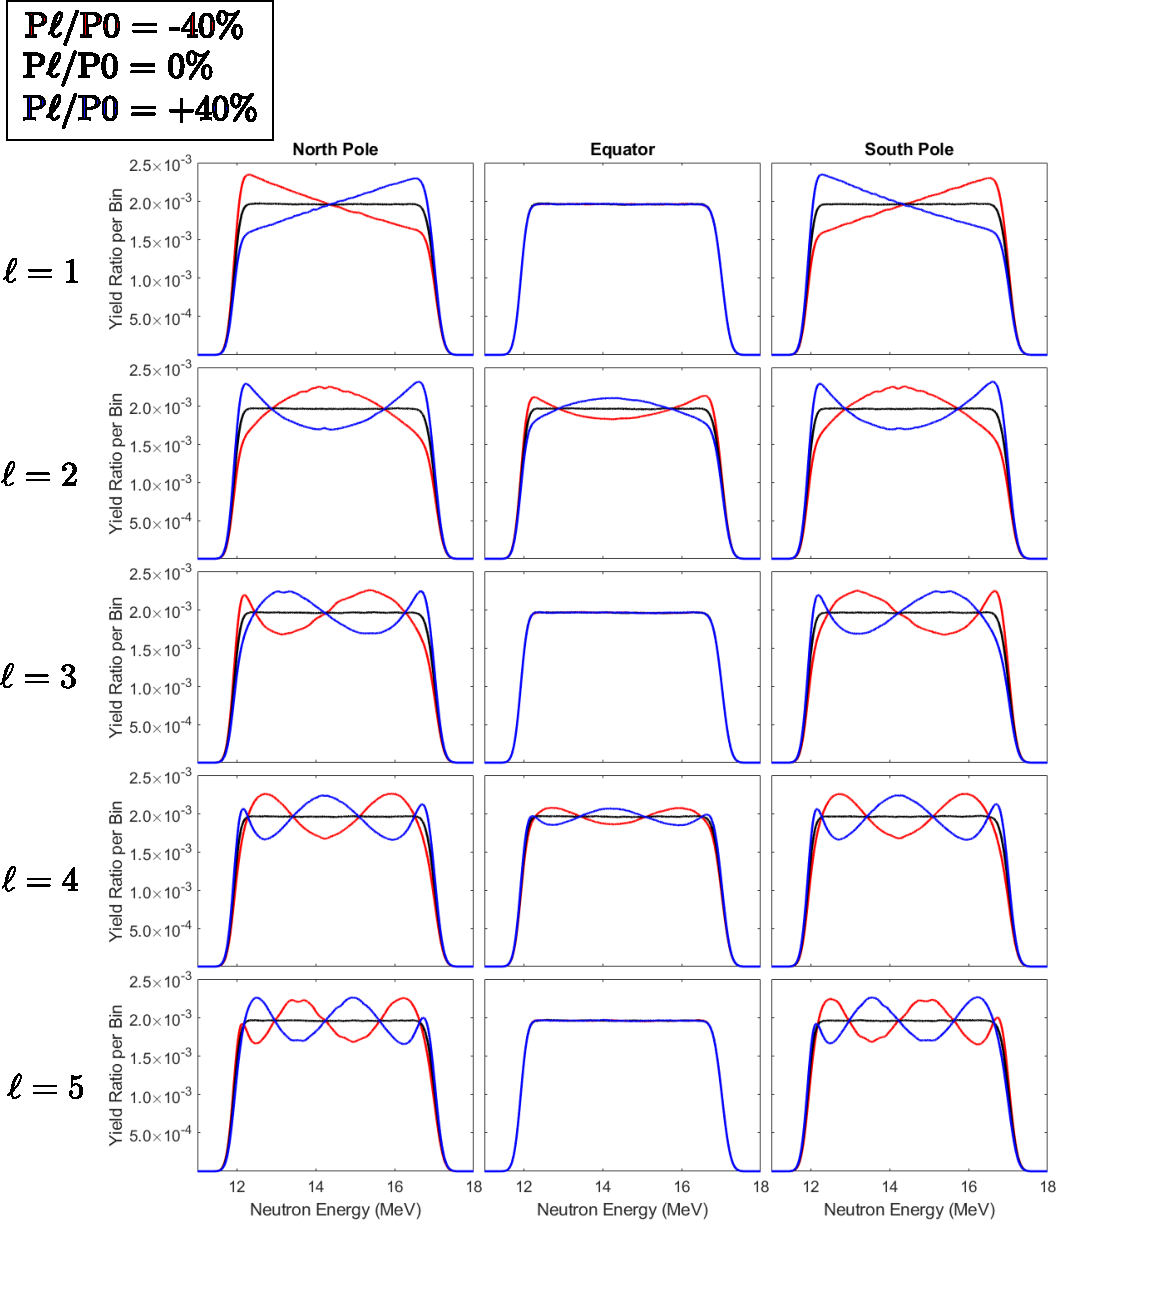
\includegraphics[scale=0.8]{Figures/secondaryDTAsymExamples.pdf}
	    \caption[Asymmetry Effects on Spectra]{Examples of secondary spectra corresponding the various plasma asymmetries. Plots in column 1,2,3 correspond to spectra as viewed from the plasmas north pole, equator, and south pole respectively. Plots in rows 1,2,3,4,5 correspond to asymetries modes 1,2,3,4, and 5 respectively. The red, black, and blue curves correspond to an asymmetry magnitude of -40\%, 0\%, and +40\% respectively. Mode magnitudes are defined in accordance to equations \ref{eq:P0} and \ref{eq:Pl}. All simulations used a uniform temperature and density of 4 keV and 1.0 g/cc respectively and all simulations had an areal density of 10 mg/cm^2. }
	    \label{fig:secondaryDTAsymExamples}
	\end{figure}
	
	    Figure \ref{fig:secondaryDTAsymExamples} shows the effects of plasma asymmetries on the observed spectra from different lines of sight. Specifically it shows the effects of low mode, azimuthually symmetric asymmetries as viewed from the north pole, the equator, and the south pole. Because the asymmetries are azimuthually symetric, the azimuthal angle of the equatorial detector is arbitrary. 
	    
	    \todo{If you find time, azimuthal asymmetries}
	    
	    As mentioned before, asymmetries are mapped onto the spectra via the relationship shown in Figure \ref{secondaryDTnEnergy}. Because of this, south pole and north pole detectors are always mirrors of one another. Also intersting is the fact that the equatorial detector is completely blind to odd mode asymmetries. 
	
	
